\paragraph{Graphical representation} Neural networks are composed of nodes (neurons), connected by direct links (synaptic connections). If we think of neurons as vertices and synaptic connections as edges, neural networks can be represented by weighted directed graphs called \textbf{network diagrams}.

If the network is feedforward (without cycles), the graph will be $ k $-partide, where $ k $ is the number of layers. If it is also fully-connected, it will be a complete $ k $-partide graph. See Figure \ref{fig:graphs} for specific examples.

\begin{figure}[H]
  \centering
  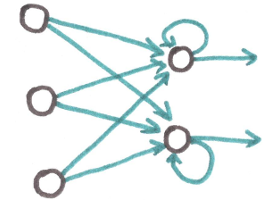
\includegraphics[width=0.3\textwidth]{recurrent}
  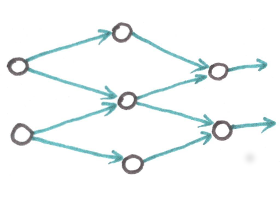
\includegraphics[width=0.3\textwidth]{feedfwd}
  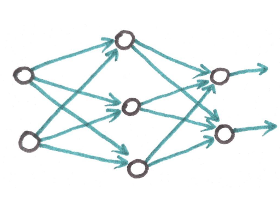
\includegraphics[width=0.3\textwidth]{full_feedfwd}
  %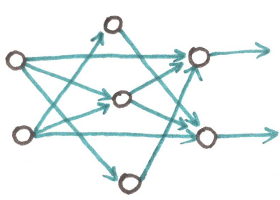
\includegraphics[width=0.4\textwidth]{nonpart_feedfwd}
  \caption{(1) Recurrent neural network represented by directed graph. (2) 3-layered feedforward neural network represented by 3-partide directed graph. (3) 3-layered fully-connected feedforward neural network represented by a complete 3-partide directed graph}
  \label{fig:graphs}
\end{figure}

\paragraph{Network topologies}
As it was already said, neural networks consist of neurons. These neurons are connected with directed links (synaptic connections) with numeric weights that determine the strength and sign of the connection.

Neurons are grouped into layers. First layer is called \textbf{input layer}, the last one - \textbf{output layer}. All the layers between input and output layers are called \textbf{hidden layers}. Number of hidden layers is one of the tunable metaparameters that define the architecture of a neural network. According to \cite{Hastie-et-al-2013}, typically the number of hidden units is somewhere in the range of 5-100.

To satisfy the linear model of a regression each layer, except for the output one, has an additional bias unit $ b = 1 $.

For a specific example of neural network architecture see Figure \ref{fig:net}.

By the type of connections neural network can be either feedforward or recurrent:
\begin{itemize}
  \item \textbf{Feedforward network} - has connections only in one direction (outputs of neurons from layer $ k $ can be connected only to neurons of layers $ k + c $ where $ c > 0 $). The network diagram of a feedforward netwond forms a directed acyclic graph.
  \item \textbf{Recurrent network} - feeds its outputs to its own inputs. This network has at least one cycle (at least one connection from neuron in layer $ k $ to neuron in layer $ k - c $ where $ c \geq 0 $). 
\end{itemize}
  
If in neural network with $ N $ layers $ \forall k:0 \leq k \leq N-1  $ every neuron in layer $ k $ is connected to all the neurons of layer $ k+1 $, the network is called \textbf{fully-connected}.
  
Figure \ref{fig:net} depicts the schematic of a feedforward neural network with one hidden layer.
  
\begin{figure}[H]
  \centering
  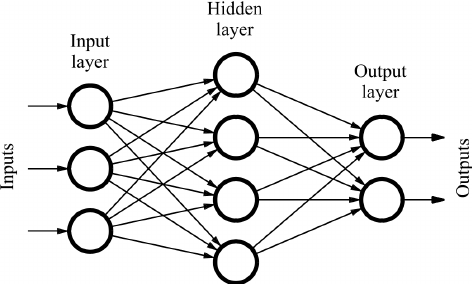
\includegraphics[width=\imgwidth]{net}
  \caption{Feedforward artificial neural network with one hidden layer. Number of neurons in each layer: 3 (2-dimentional input + bias unit) in the input layer, 4 in the hidden layer, 1 in the output layer (1-demensional output)}
  \label{fig:net}
\end{figure}
